\label{ch:introduction}

One of the tasks associated with being a real estate agent is to determine how much property is worth in order to set a price that is not so high that the property will not receive any interest, but not so low that the full potential is not utilized.
% \textbf{Housing prices depends on different factors.}
The price of a house depend on many factors both internal and external.
Internal factors could refer to the size, condition or layout.
External factors could refer to the were the property is located, interest rates or economic growth.
% \textbf{Different factors for different types of housing.}
For different types of property only certain factors are applicable.
Take for instance the apartment market where the size of the lot is a not applicable factor.
To create a statistical model based on applicable factors, these factors must be measurable.
An easily measurable factor is the size in $m^2$, as this is a objective measure which is universal.
But there is other factors such as the condition, this is a non-universal factor.
One person might find an apartment to be in great condition, whereas another might find the same apartment to be in poor condition.
% \textbf{Factors must be measureable.}
So this is one possible consideration to take into account when considering which factors to consider including in a statistical model.
% \textbf{Apartments are more homogenous.}
In relation to the above considerations one might split the housing market into different segments and consider these as separate markets.
Take for instance the apartment market, some of the internal factors are size, condition, balcony and so on.
Consider next the market for single family homes, this market is affected for instance by the additional internal factor lot size.
This is an additional factor that blurs the widely used metric of price per square meter of living space.
To illustrate suppose all else equal two identical homes on different sized lots, then one house might have a higher price per square meter as it sits on a larger lot which might be more expensive.
Thus we have to control for lot size in our statistical model.
But then the gardens might be of different condition, which we would have to control for as well.
Because of these additional consideration which will have to be made regarding the market for single family homes, the market for apartment is inherently more homogeneous.
In other words there are less factors to consider in the market for apartments.


\section{Data Introduction}
In this section we will explore the dataset from HOME that is to be analysed in this project.
The dataset consists of information regarding property sales in the period from 2004 to 2016.
It has 131.920 observations where the price as well as some additional information on the property in question has been recorded.
Following a preliminary examination of the dataset, we have chosen to focus on apartments in the four largest danish cities. 
These being Copenhagen, Aarhus, Odense and Aalborg.
For the variables we have chosen to focus on
%\begin{multicols}{2}
\begin{enumerate}
    \item City
    \item Property Condition
    % \begin{itemize}[label = -]
    %     \item A qualitative evaluation of the condition of the property which can fall in one of three categories; ``Bad'', ``Okay'', ``Good''.
    % \end{itemize}
    \item Size in $m^2$
    % \begin{itemize}[label = -]
    %     \item The number of square meters that represents actual living space whitin the property. 
    % \end{itemize}
    \item Year of sale
    \item Selling period in days
    % \begin{itemize}[label = -]
    %     \item Number of days between the day the property went on the market and the day the property was sold.
    % \end{itemize}
    \item Year of construction
    \item Balcony or not
    % \begin{itemize}[label = -]
    %     \item A binary variable that tells whether or not the property have a balcony.
    % \end{itemize}
    \item Renovation or not
    % \begin{itemize}[label = -]
    %     \item A binary variable that tells if the property have ever been renovated.
    % \end{itemize}
\end{enumerate}
%\end{multicols}
Restricting to the cities in question results in a reduction of the number of observations.
Furthermore we have chosen to disregard observations that contain NA values.
The number of observations after the reduction is 3.086.

\section{Partitioning the Dataset}
In preparation for section \ref{sec:prediction} we will set aside the observations from sales in 2016.
These observations can then be used to asses the predictive accuracy of the models that will be developed in the project.
The number of sales in 2016 amounts to 200 observations, the distribution between cities can be found in table \ref{tbl:2016_obs_per_city}.
\begin{table}[H]
    \centering
    \begin{tabular}{lr}
        \toprule
        \textbf{City} & \textbf{Obs.}\\
        \midrule
        Copenhagen & 108\\
        Odense & 27\\
        Aalborg & 19\\
        Aarhus & 46\\
        \bottomrule
    \end{tabular}
    \caption{Count of apartments sold in 2016 per city.}
    \label{tbl:2016_obs_per_city}
\end{table}
In the next section we will investigate the remaining observations from the dataset, i.e. the observations that were sold between 2004 and 2016.

\section{Descriptive Statistics}
This section will provide a brief summary for each of the variables.
But first we can take a look at the price which will be treated as the dependent variable in this project.
In table \ref{tbl:summary_of_price} a summary of the apartment prices can be seen.
In table \ref{tbl:summary_of_price}, \textbf{Q1} and \textbf{Q3} represents the first and third quartile respectively.
\begin{table}[H]
    \centering
    \begin{tabular}{rrrrrrr}
        \toprule
        \textbf{minimum} & \textbf{Q1} & \textbf{median} & \textbf{mean} & \textbf{Q3} & \textbf{maximum} & \textbf{std. deviation}\\
        \midrule
        200\:000 & 1\:175\:000 & 1\:725\:000 & 2\:069\:337 & 2\:600\:000 & 15\:550\:000 & 1\:302\:274\\
        \bottomrule
    \end{tabular}
    \caption{Summary of apartment prices.}
    \label{tbl:summary_of_price}
\end{table}
To further investigate the distribution of the price a histogram of the apartment prices has been plotted in figure \ref{fig:histogram_of_price}.
As is evident on the plot, the price is clearly left skewed.
This is expected as the median is below the mean.
\begin{figure}[H]
    \centering
    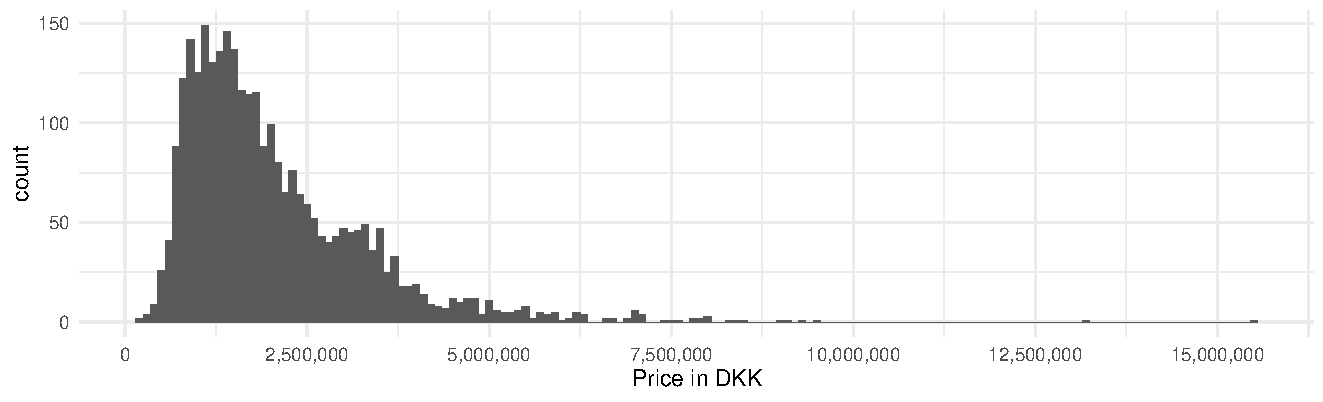
\includegraphics[width=0.9\textwidth]{figures/Data_introduction/price_histogram.pdf}
    \caption{A histogram of the apartment price with a binwidth of 100\:000 DKK.}
    \label{fig:histogram_of_price}
\end{figure}

\subsection*{City}
How the observations are distributed between the cities can be seen on figure \ref{fig:distributions_between_cities}.
\begin{figure}[H]
    \centering
    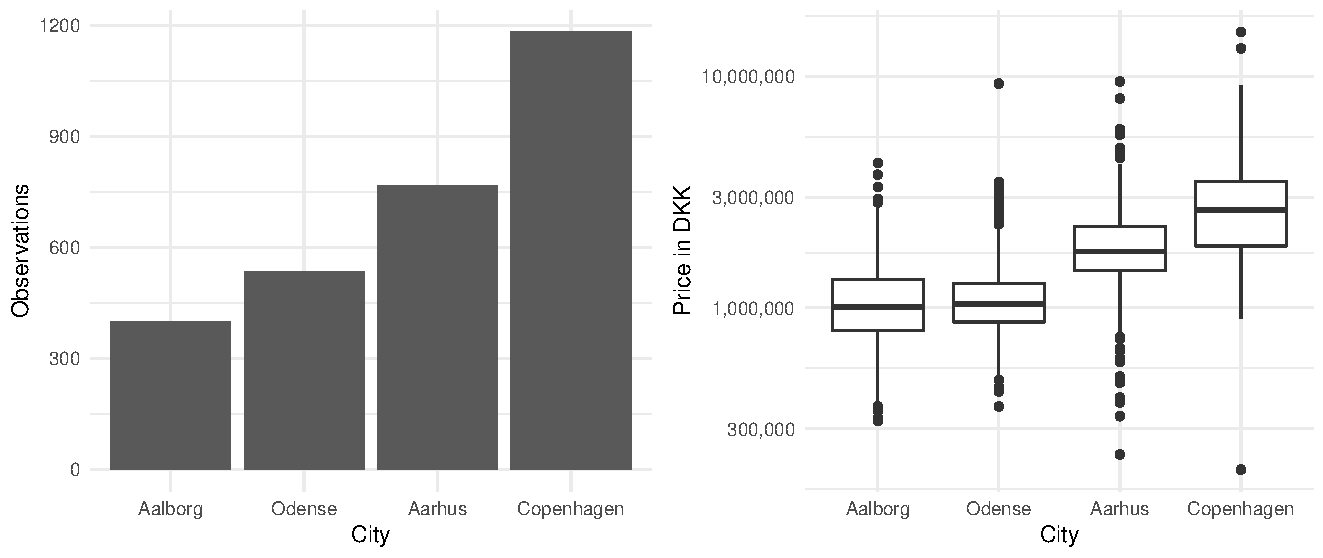
\includegraphics[width=0.9\textwidth]{figures/Data_introduction/distribution_between_cities.pdf}
    \caption{Distribution of observations and a boxplot of price between the cities.}
    \label{fig:distributions_between_cities}
\end{figure}
Here it is seen that most observations are from Copenhagen, which is to be expected as there are more apartments than in the other 3 cities.
The differences in the average price between the cities indicate that, this may influence the selling price.

\subsection*{Quality of property}
A qualitative evaluation of the condition of the property which can fall in one of three categories; ``Low'', ``Medium'', ``High''.
A count of the 2.886 total observations in each of the categories can be found in table \ref{tbl:property_condition}.
\begin{table}[H]
    \centering
    \begin{tabular}{lr}
        \toprule
        \textbf{Property Condition} & \textbf{Obs.}\\
        \midrule
        Low & 86\\
        Medium & 1472\\
        High & 1328\\
        \bottomrule
    \end{tabular}
    \caption{Count of observations per property condition.}
    \label{tbl:property_condition}
\end{table}
It is notable that there are very few observations in the ``Low'' category, compared to the other two. 
This variable may not prove very useful since every category is so large.

\subsection*{Size in \textit{m}$\mathbf{^2}$}
This variable measures the size of the property in square meters.
\begin{table}[H]
    \centering
    \begin{tabular}{rrrrrrr}
        \toprule
        \textbf{minimum} & \textbf{Q1} & \textbf{median} & \textbf{mean} & \textbf{Q3} & \textbf{maximum} & \textbf{std. deviation}\\
        \midrule
        12 & 59 & 75 & 81.42238 & 94 & 438 & 33.30229\\
        \bottomrule
    \end{tabular}
    \caption{Summary of the ``size in $m^2$'' variable.}
    \label{tbl:size_in_m2}
\end{table}
A widely used measure for the price of a house is the price per square meter.
In figure \ref{fig:price_per_square_meter} the relationship between the selling price and size of apartments is illustrated.
The figure shows a clear positive relationship between the two variables in all of the four cities.
\begin{figure}[H]
    \centering
    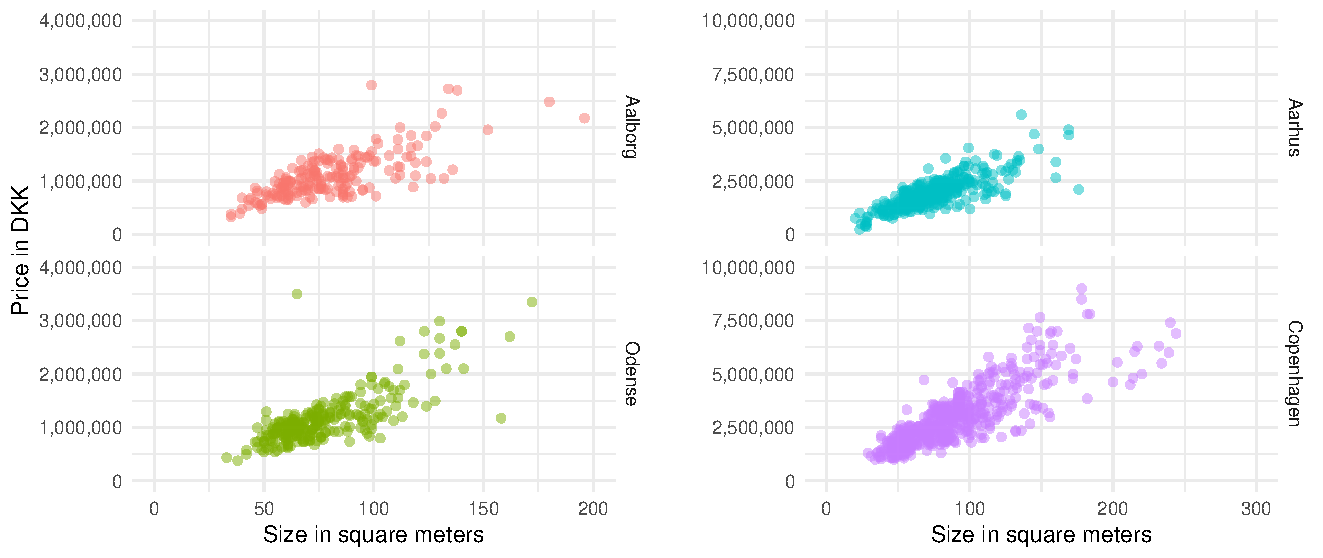
\includegraphics[width=\textwidth]{figures/Data_introduction/price_per_square_meter.pdf}
    \caption{Relationship between the selling price and size of apartments in the four cities.}
    \label{fig:price_per_square_meter}
\end{figure}

\subsection*{Year of Sale}
This variable is a categorical variable that can take one of three possible outcomes, namely ``pre.crisis'', ``crisis'' or ``post.crisis''.
In table \ref{tbl:year_of_sale} a count of observations in each of the categories can be found.
\begin{table}[H]
    \centering
    \begin{tabular}{lr}
        \toprule
        \textbf{Year of Sale} & \textbf{Obs.}\\
        \midrule
        pre.crisis & 1008\\
        crisis & 1001\\
        post.crisis & 877\\
        \bottomrule
    \end{tabular}
    \caption{Count of observations per year of sale category.}
    \label{tbl:year_of_sale}
\end{table}

In figure \ref{fig:year_of_sale_histogram} it can be seen how the distribution of sales have been in the period from 2004 to 2016.
\begin{figure}[H]
    \centering
    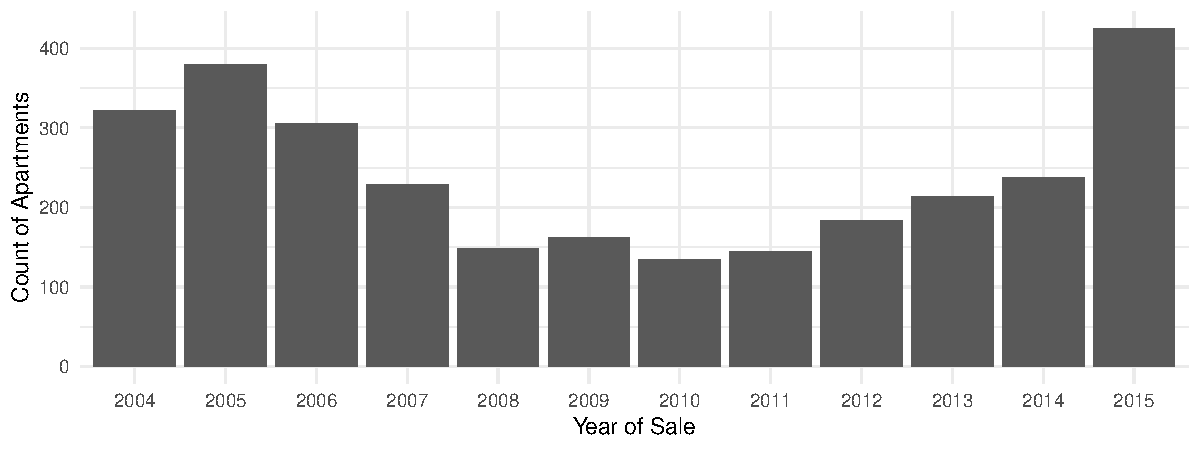
\includegraphics[width = 0.8 \textwidth]{figures/Data_introduction/year_of_sale_histogram.pdf}
    \caption{Histogram showing how many sales there have been per year.}
    \label{fig:year_of_sale_histogram}
\end{figure}
% \begin{table}[H]
%     \centering
%     \begin{tabular}{lr|lr|lr}
%         \toprule
%         \multicolumn{2}{c}{\textbf{2004-2008}} & \multicolumn{2}{c}{\textbf{2009-2013}} &
%         \multicolumn{2}{c}{\textbf{2014-2015}} \\
%         \toprule
%         \textbf{Year of sale} & \textbf{Obs.} & 
%         \textbf{Year of sale} & \textbf{Obs.} & 
%         \textbf{Year of sale} & \textbf{Obs.}\\
%         \midrule
%         2004 & 322 & 2009 & 162 & 2014 & 238\\   
%         2005 & 380 & 2010 & 134 & 2015 & 425\\   
%         2006 & 306 & 2011 & 144\\   
%         2007 & 229 & 2012 & 184\\   
%         2008 & 148 & 2013 & 214\\   
%         \bottomrule
%     \end{tabular}
%     \caption{Summary of the ``Year of sale'' variable.}
%     \label{tbl:year_of_sale}
% \end{table}
As mentioned the dataset includes house sales in the period from 2004 to 2016.
Naturally there will be some fluctuations in the average price from one year to another, just as a result of the economic cycle.
Especially the years during the financial crisis a fall in the average selling price is expected.
Indeed it is also possible to see this trend in the data as figure \ref{fig:house_price_year} suggest.

\subsection*{Selling Period}
This is a variable that counts the number of days it took to sell the apartment.
If the value is 0 the apartment was either sold the day it went on the market or it might not even have been on the market.
\begin{table}[H]
    \centering
    \begin{tabular}{rrrrrrr}
        \toprule
        \textbf{minimum} & \textbf{Q1} & \textbf{median} & \textbf{mean} & \textbf{Q3} & \textbf{maximum} & \textbf{std. deviation}\\
        \midrule
        0 & 27 & 62.5 & 97.7079 & 131.75 & 1321 & 112.5781\\
        \bottomrule
    \end{tabular}
    \caption{Days until the property was sold.}
    \label{tbl:days_until_sold}
\end{table}

\subsection*{Decade of Construction}
The dataset has information regarding which year the apartment have been constructed.
We have here chosen to group the variable in decades.
In table \ref{tbl:year_of_constuction} there is a count of apartments constructed per decade.
\begin{table}[H]
    \centering
    \begin{tabular}{lr|lr|lr|lr|lr}
        \toprule [1.5pt]
        \multicolumn{2}{c}{\textbf{1800-1840}} & 
        \multicolumn{2}{c}{\textbf{1850-1890}} & 
        \multicolumn{2}{c}{\textbf{1900-1940}} & 
        \multicolumn{2}{c}{\textbf{1940-1990}} & 
        \multicolumn{2}{c}{\textbf{2000-2010}} \\[2pt]
        \toprule[1.5pt]
        \textbf{Year} & \textbf{Obs.} & 
        \textbf{Year} & \textbf{Obs.} & 
        \textbf{Year} & \textbf{Obs.} & 
        \textbf{Year} & \textbf{Obs.} & 
        \textbf{Year} & \textbf{Obs.} \\
        \midrule
        1800 & 88 & 1850 & 46  & 1900 & 305 & 1950 & 231 & 2000 & 145 \\
        1810 & 20 & 1860 & 28  & 1910 & 163 & 1960 & 166 & 2010 & 160 \\
        1820 & 6  & 1870 & 89  & 1920 & 144 & 1970 & 74  \\
        1830 & 14 & 1880 & 164 & 1930 & 585 & 1980 & 71  \\
        1840 & 39 & 1890 & 227 & 1940 & 97  & 1990 & 24  \\
        \bottomrule
    \end{tabular}
    \caption{Count of observation per decade of construction}
    \label{tbl:year_of_constuction}
\end{table}
An interesting pattern in the data is how the selling price is affected by the year of construction.
A possible intuition would be that the newer the apartment the higher the selling price, however the data suggests another pattern as is evident in figure \ref{fig:house_price_year}.

\begin{figure}[H]
    \centering
    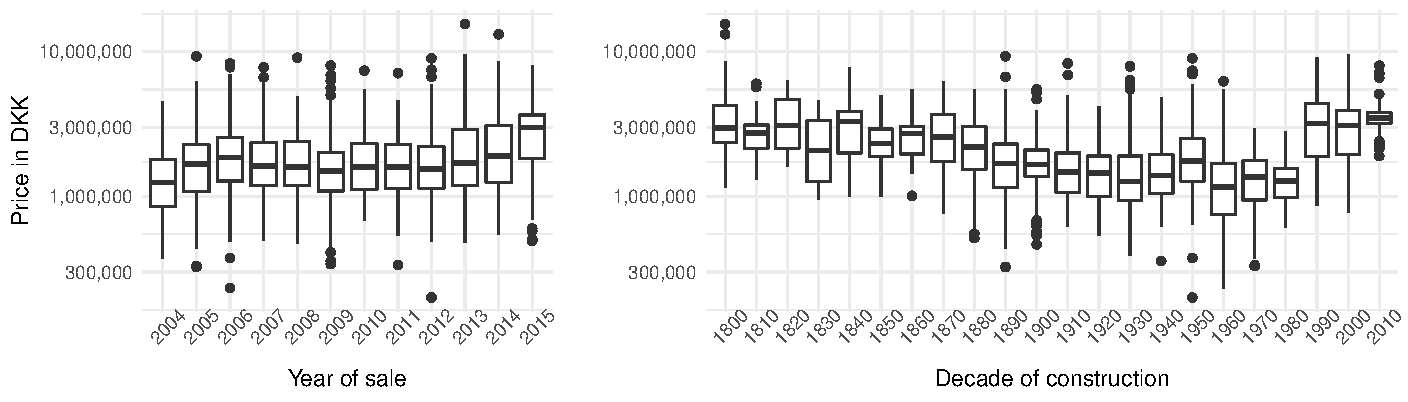
\includegraphics[width = \textwidth]{figures/Data_introduction/house_price_year.pdf}
    \caption{A boxplot of the average selling price against the year of sale and the decade of construction respectively.}
    \label{fig:house_price_year}
\end{figure}
The pattern suggested is that new apartments as well as old apartment have the highest mean price, whereas the apartments constructed from the 1890's until the 1980's have a lower mean price.
However there could be other factors to account for.

\subsection*{Balcony and Renovation}
The variables regarding whether the apartment has a balcony or has been renovated are binary.
This means that they can take either the value 0 or 1, where 0 refers to the case where the apartment does not have a balcony or has not been renovated and vice versa.
\begin{table}[H]
    \centering
    \begin{tabular}{lr}
        \toprule
        \textbf{Balcony or not} & \textbf{Obs.}\\
        \midrule
        0 & 1508\\
        1 & 1378\\
        \bottomrule
    \end{tabular}
    \hspace{20pt}
    \begin{tabular}{lr}
        \toprule
        \textbf{Renovation or not} & \textbf{Obs.}\\
        \midrule
        0 & 2329\\
        1 & 557\\
        \bottomrule
    \end{tabular}
    \caption{Count of observations per balcony and renovation.}
\end{table}

\section{Predictive Performance}
\textbf{Predictive performance, essential for HOME.}

\section{Statement of Intent}
Here the statement of intent is supposed to go.